\documentclass[border=8pt]{standalone}
\usepackage{amsmath,amssymb}
\usepackage{tikz}
\usetikzlibrary{arrows.meta,calc,decorations.pathreplacing,patterns,shapes.geometric,positioning,shadings,plotmarks}

\begin{document}
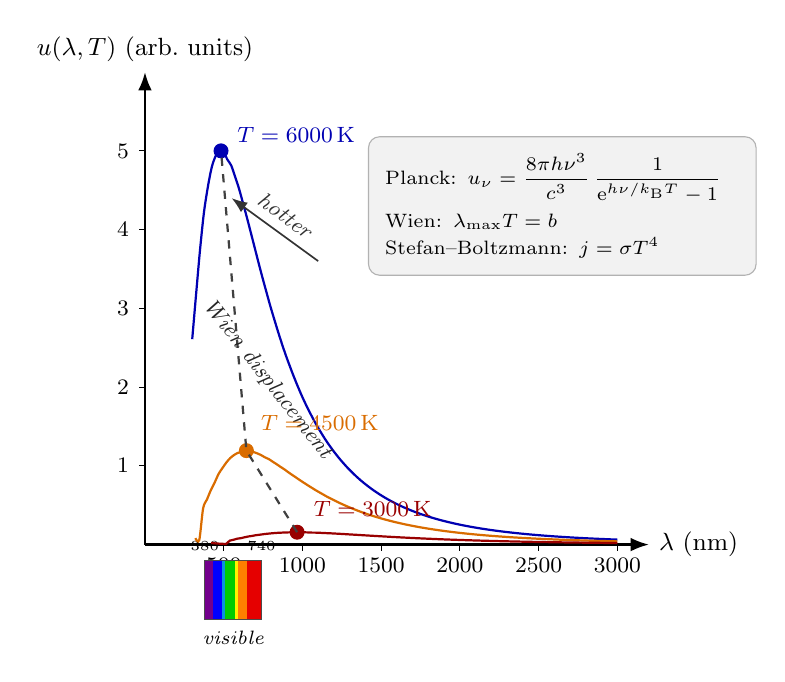
\begin{tikzpicture}[>=Latex, scale=1.0]

% =====================================================
% Blackbody Planck curves for T = 3000, 4500, 6000 K
% x = lambda in micrometers; x = 1 um -> 2 cm on plot
% Using stable form:
%   E = exp(-14.388 / (x*T_k))
%   u = K * x^{-5} * E / (1 - E),  with K = 18.73 chosen so 6000 K peak ~ 5.0
% Peak positions (lambda_max T = 2898 um*K):
%   T=6000 K: 0.483 um (483 nm)
%   T=4500 K: 0.644 um (644 nm)
%   T=3000 K: 0.966 um (966 nm)
% =====================================================

\def\xmax{3.0}
\def\ymax{5.5}

% --- Axes ---
\draw[->, thick] (0,0) -- (\xmax*2 + 0.4, 0)
  node[right, font=\small] {$\lambda\ (\mathrm{nm})$};
\draw[->, thick] (0,0) -- (0, \ymax + 0.5)
  node[above, font=\small] {$u(\lambda,T)$ (arb.\ units)};

% X ticks every 500 nm (x in um; plot unit 1 um = 2 cm)
\foreach \xn/\lab in {0.5/500, 1.0/1000, 1.5/1500, 2.0/2000, 2.5/2500, 3.0/3000} {
    \draw (\xn*2, 0) -- (\xn*2, -0.08);
    \node[below, font=\footnotesize] at (\xn*2, -0.05) {\lab};
}

% Y-axis ticks
\foreach \yn in {1,2,3,4,5} {
    \draw (0, \yn) -- (-0.08, \yn);
    \node[left, font=\footnotesize] at (-0.08, \yn) {\yn};
}

% --- Visible rainbow band below x-axis: 380..740 nm, i.e. x in [0.38,0.74] um ---
% Plot coords: x*2 so [0.76, 1.48]
\fill[violet!90!blue]  (0.76, -0.95) rectangle (0.86, -0.20); % 380-430 violet
\fill[blue]            (0.86, -0.95) rectangle (0.98, -0.20); % 430-490 blue
\fill[cyan!80!blue]    (0.98, -0.95) rectangle (1.02, -0.20); % 490-510 cyan
\fill[green!80!black]  (1.02, -0.95) rectangle (1.14, -0.20); % 510-570 green
\fill[yellow]          (1.14, -0.95) rectangle (1.18, -0.20); % 570-590 yellow
\fill[orange]          (1.18, -0.95) rectangle (1.30, -0.20); % 590-650 orange
\fill[red!90!black]    (1.30, -0.95) rectangle (1.48, -0.20); % 650-740 red
\draw[thin, gray!60!black] (0.76, -0.95) rectangle (1.48, -0.20);
\node[font=\scriptsize\itshape, below] at (1.12, -0.97) {visible};

% Mark 380 and 740 on rainbow band
\node[font=\tiny, above] at (0.76, -0.20) {380};
\node[font=\tiny, above] at (1.48, -0.20) {740};

% =====================================================
% Planck curves using numerically stable sampled form
% u(x,T) = 18.73 / ( x^5 * (exp(14.388/(x*Tk)) - 1) )
% =====================================================

% We use the numerically stable form:
%   u = 18.73 * exp(-a/(xT)) / ( x^5 * (1 - exp(-a/(xT))) )
% with a = 14.388.  This avoids huge intermediate values because
% exp(-a/(xT)) is always <= 1.

% T=6000 K (cool blue, hottest)
\draw[thick, blue!70!black, smooth, samples=110, domain=0.30:3.0, variable=\x]
  plot ({\x*2},
        { 18.73 * exp(-14.388/(\x*6)) /
          ( (\x*\x*\x*\x*\x) * ( 1 - exp(-14.388/(\x*6)) ) ) });

% T=4500 K (orange, middle)
\draw[thick, orange!85!black, smooth, samples=110, domain=0.32:3.0, variable=\x]
  plot ({\x*2},
        { 18.73 * exp(-14.388/(\x*4.5)) /
          ( (\x*\x*\x*\x*\x) * ( 1 - exp(-14.388/(\x*4.5)) ) ) });

% T=3000 K (deep red, coolest)
\draw[thick, red!60!black, smooth, samples=110, domain=0.42:3.0, variable=\x]
  plot ({\x*2},
        { 18.73 * exp(-14.388/(\x*3)) /
          ( (\x*\x*\x*\x*\x) * ( 1 - exp(-14.388/(\x*3)) ) ) });

% --- Peak dots ---
\filldraw[blue!70!black]   (0.966, 5.00)  circle (2.5pt);
\filldraw[orange!85!black] (1.288, 1.193) circle (2.5pt);
\filldraw[red!60!black]    (1.932, 0.157) circle (2.5pt);

% --- Dashed line connecting peaks (Wien displacement) ---
\draw[dashed, gray!50!black, thick]
  (1.932, 0.157) -- (1.288, 1.193) -- (0.966, 5.00);

\node[rotate=-52, font=\footnotesize\itshape, text=gray!30!black]
  at (1.55, 2.1) {Wien displacement};

% --- Curve labels ---
\node[font=\footnotesize, blue!70!black, anchor=west]
  at (1.05, 5.20) {$T=6000\,\mathrm{K}$};
\node[font=\footnotesize, orange!85!black, anchor=west]
  at (1.35, 1.55) {$T=4500\,\mathrm{K}$};
\node[font=\footnotesize, red!60!black, anchor=west]
  at (2.02, 0.45) {$T=3000\,\mathrm{K}$};

% --- Arrow "hotter" pointing toward shorter wavelengths ---
\draw[->, semithick, gray!40!black] (2.2, 3.6) -- (1.1, 4.4)
  node[midway, above, sloped, font=\footnotesize\itshape] {hotter};

% --- Formula box (top right) ---
\node[draw=gray!60, fill=gray!10, rounded corners, align=left,
      font=\scriptsize, text width=4.5cm, inner sep=6pt]
  at (5.3, 4.3) {%
    Planck: $\displaystyle u_\nu=\frac{8\pi h\nu^{3}}{c^{3}}\,
       \frac{1}{\mathrm{e}^{h\nu/k_{\mathrm{B}}T}-1}$ \\[3pt]
    Wien: $\lambda_{\max}T = b$ \\[2pt]
    Stefan--Boltzmann: $j = \sigma T^{4}$
  };

\end{tikzpicture}
\end{document}
